\def\duedate{\today}
\def\HWnum{3}
\documentclass[10pt,a4paper]{book}

% custom section formatting
\usepackage{titlesec}
\titleformat{\chapter}[display]
{\normalfont\Large\filcenter\sffamily}
{\titlerule[1pt]%
\vspace{1pt}%
\titlerule
\vspace{1pc}%
\LARGE\MakeUppercase{\chaptertitlename} \thechapter}
{1pc}
{\titlerule
\vspace{1pc}%
\Huge}

% appendix handling
\usepackage[toc,page]{appendix}
    
% encoding for file and font
\usepackage[utf8]{inputenc}
\usepackage[T1]{fontenc}

% math formatting/tools
\usepackage{amsmath}
\usepackage{amssymb}
\usepackage{mathtools}
\usepackage[arrowdel]{physics}

% unit formatting
\usepackage{siunitx}
\AtBeginDocument{\RenewCommandCopy\qty\SI}

% figure formatting/tools
\usepackage{graphicx}
\usepackage{float}
\usepackage{subcaption}
\usepackage{multirow}
\usepackage{import}
\usepackage{pdfpages}
\usepackage{transparent}
\usepackage{currfile}

\NewDocumentCommand\incfig{O{1} m}{
    \def\svgwidth{#1\textwidth}
    \import{./Figures/\currfiledir}{#2.pdf_tex}
}

\newcommand{\bef}{\begin{figure}[h!tb]\centering}
\newcommand{\eef}{\end{figure}}

\newcommand{\bet}{\begin{table}[h!tb]\centering}
\newcommand{\eet}{\end{table}}

% hyperlink references 
\usepackage{hyperref}
\hypersetup{
    colorlinks=true,
    linkcolor=blue,
    filecolor=magenta,
    urlcolor=cyan,
    pdftitle={Physics 1 Notes},
    pdfauthor={Richard Whitehill},
    pdfpagemode=FullScreen
}
\urlstyle{same}

\newcommand{\eref}[1]{Eq.~(\ref{eq:#1})}
\newcommand{\erefs}[2]{Eqs.~(\ref{eq:#1})--(\ref{eq:#2})}

\newcommand{\fref}[1]{Fig.~(\ref{fig:#1})}
\newcommand{\frefs}[2]{Fig.~(\ref{fig:#1})--(\ref{fig:#2})}

\newcommand{\aref}[1]{Appendix~(\ref{app:#1})}
\newcommand{\sref}[1]{Section~(\ref{sec:#1})}
\newcommand{\srefs}[2]{Sections~(\ref{sec:#1})-(\ref{sec:#2})}

\newcommand{\tref}[1]{Table~(\ref{tab:#1})}
\newcommand{\trefs}[2]{Table~(\ref{tab:#1})--(\ref{tab:#2})}

% tcolorbox formatting/definitions
\usepackage[most]{tcolorbox}
\usepackage{xcolor}
\usepackage{xifthen}
\usepackage{parskip}

\definecolor{peach}{rgb}{1.0,0.8,0.64}

\DeclareTColorBox[auto counter, number within=chapter]{defbox}{O{}}{
    enhanced,
    boxrule=0pt,
    frame hidden,
    borderline west={4pt}{0pt}{green!50!black},
    colback=green!5,
    before upper=\textbf{Definition \thetcbcounter \ifthenelse{\isempty{#1}}{}{: #1} \\ },
    sharp corners
}

\newcommand*{\eqbox}{\tcboxmath[
    enhanced,
    colback=black!10!white,
    colframe=black,
    sharp corners,
    size=fbox,
    boxsep=8pt,
    boxrule=1pt
]}

\newtcolorbox[auto counter, number within=chapter]{exbox}{
    parbox=false,
    breakable,
    enhanced,
    sharp corners,
    boxrule=1pt,
    colback=white,
    colframe=black,
    before upper= \textbf{Example \thetcbcounter:}\,,
    before lower= \textbf{Solution:}\,,
    segmentation hidden
}

\newtcolorbox{resbox}{
    enhanced,
    colback=black!10!white,
    colframe=black,
    boxrule=1pt,
    boxsep=0pt,
    top=2pt,
    ams nodisplayskip,
    sharp corners
}


\begin{document}

\prob{1}{

A point charge $q$ is brought to a position a distance $d$ away from an infinite plane conductor held at zero potential.
Using the method of images, find: \\[1pt]

(a) the surface-charge density induced on the plane, and plot it;

(b) the force between the plane and the charge by using Coulomb's law for the force between the charge and its image;

(c) the total force acting on the plane by integrating $\sigma^2 / 2 \epsilon_0$ over the whole plane;

(d) the work necessary to remove the charge $q$ from its position to infinity;

(e) the potential energy between the charge $q$ and its image [compare the answer to part(d) and discuss];

(f) Find the answer to part (d) in electron volts for an electron originally one angstrom from the surface.

}

\begin{figure}[h!]
   \centering
   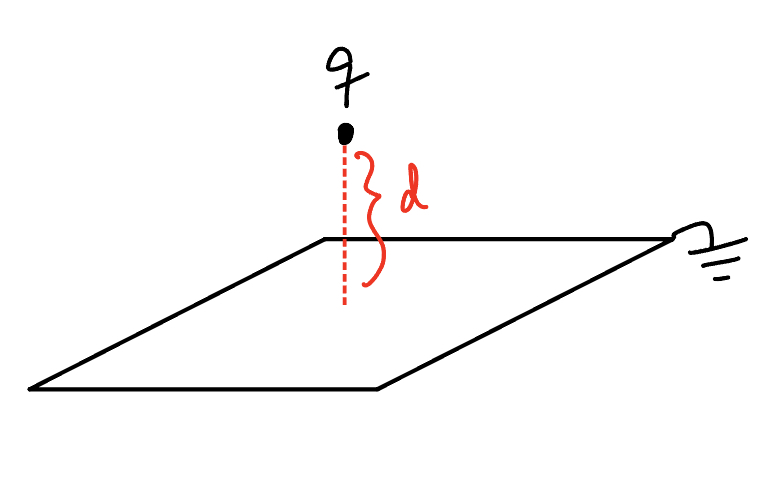
\includegraphics[width=0.4\textwidth]{prob1.jpeg}
   \caption{Sketch of setup with charge $q$ brought to a distance $d$ from an infinite grounded, conducting plane.}
   \label{fig:prob1}
\end{figure}

\sol{

(a) Solving this problem using the method of images, we place an image charge $-q$ on the other side of the plane a distance $d$ away.
The potential of this setup is
\begin{eqnarray}
    \Phi(\va*{r}) = \frac{q}{4 \pi \epsilon_0} \Bigg( \frac{1}{|\va*{r} - d \vu*{e}_{z}|} - \frac{1}{|\va*{r} + d \vu*{e}_{z}|} \Bigg)
.\end{eqnarray}
We know that this is the correct potential since it satisfies Laplace's equation for $z > 0$ (defining the $z$-axis perpendicular to the plane and the $+$ direction pointing from the plane to the charge $q$) and the boundary conditions $\Phi(x,y,0) = 0$.

The relation between the potential and surface charge density is
\begin{eqnarray}
    \eqbox{
    \begin{aligned}
        \sigma &= \epsilon_0 \pdv{\Phi}{z} = \frac{q}{4 \pi} \pdv{z} \Bigg( \frac{1}{\sqrt{x^2 + y^2 + (z - d)^2}} - \frac{1}{\sqrt{x^2 + y^2 + (z + d)^2}} \Bigg)_{z = 0} \\
               &= \frac{q}{4 \pi} \Bigg( \frac{2 (z - d)}{[ x^2 + y^2 + (z - d)^2 ]^{3/2}} - \frac{2 (z + d)}{[ x^2 + y^2 + (z + d)^2 ]^{3/2}} \Bigg)_{z = 0} \\
               &= - \frac{qd}{\pi (\rho^2 + d^2)^{3/2}}
    ,\end{aligned}
}
\end{eqnarray}
where we have defined $\rho^2 = x^2 + y^2$.
Notice that the induced charge has an overall charge with sign opposite that of $q$.

\begin{figure}[h!]
   \centering
   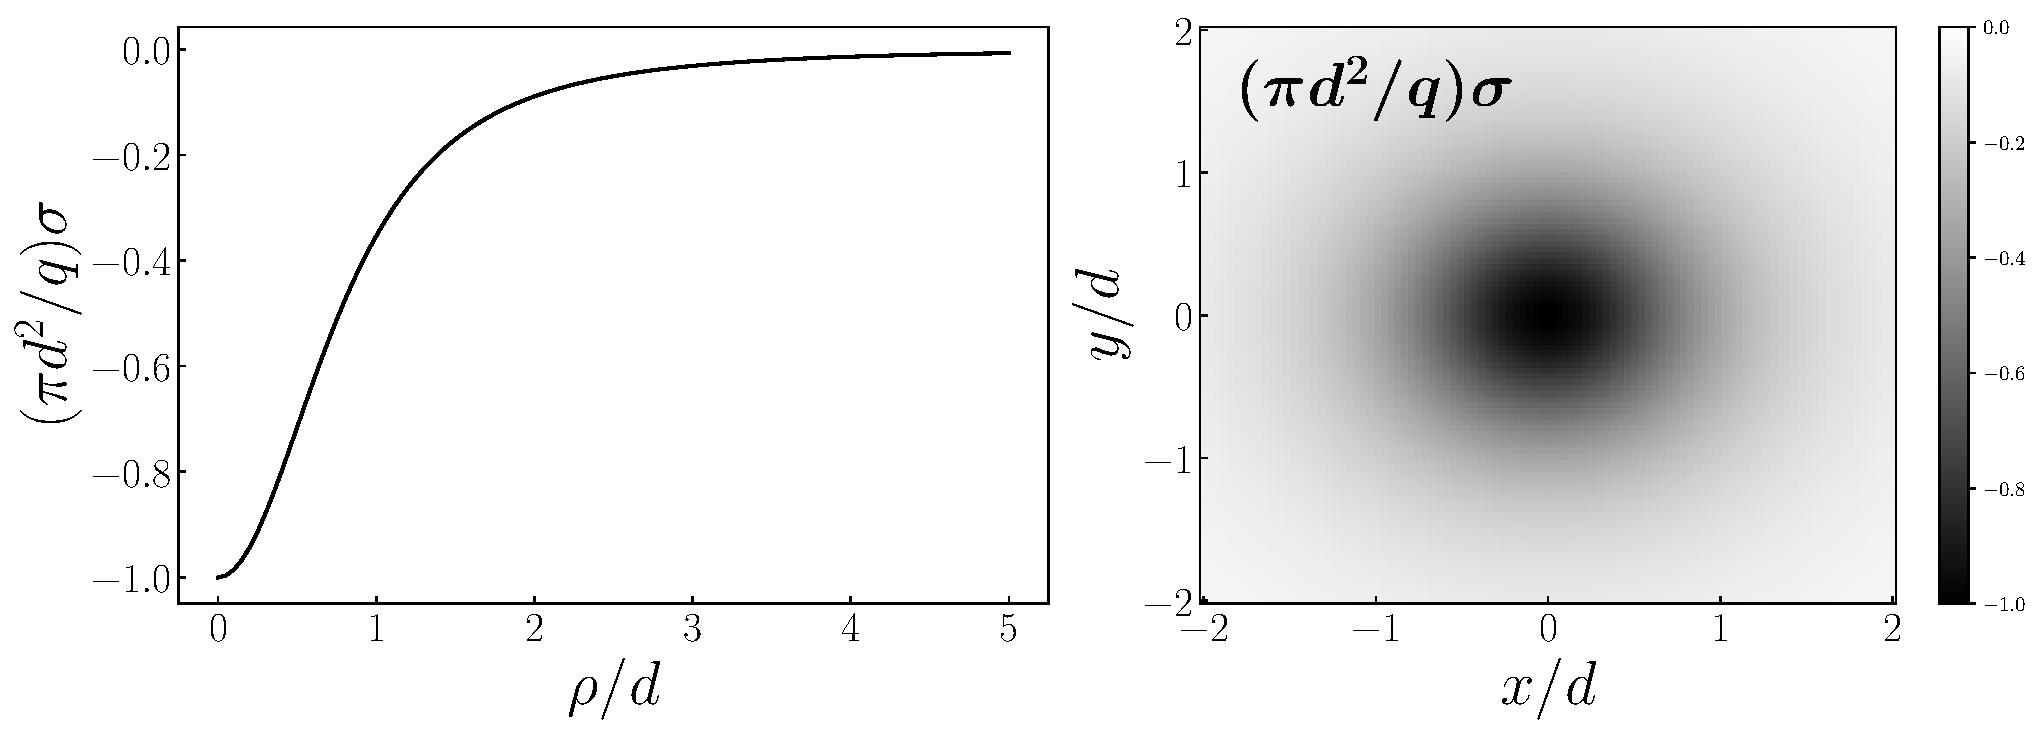
\includegraphics[width=\textwidth]{prob1a.pdf}
   \caption{\textbf{Left} -- Plot of surface charge density with respect to spatial variable $\rho = \sqrt{x^2 + y^2}$ and \textbf{Right} -- Plot of surface charge density with respect to $(x,y)$ coordinate points. Note that the spatial variables are in units of $d$, and furthermore, in the colormap plot on the right, one can intuitively read this to say that more charge aggregates directly below the charge $q$ and the distribution falls off radially from this center.}
   \label{fig:prob1a}
\end{figure}

(b) The force between the plane and point charge $q$ can be calcualted using Coulomb's law between $q$ and $-q$
\begin{eqnarray}
    \eqbox{ \va*{F} = - \frac{q^2}{4 \pi \epsilon_0} \frac{1}{2d^2} }
.\end{eqnarray}

(c) We can also calculate the total force acting on the plane as follows:
\begin{eqnarray}
    \eqbox{
   \begin{aligned}
       F &= \int \frac{\sigma^2(x,y)}{2 \epsilon_0} \dd{x} \dd{y} = \frac{q^2 d^2}{2 \pi^2 \epsilon_0} \int_{0}^{2 \pi} \int_{0}^{\infty} \frac{1}{(\rho^2 + d^2)^{3/2}} \rho \dd{\rho} \dd{\phi} \\
         &= \Big( \frac{q d}{\pi} \Big)^2 \int_{0}^{\infty} \frac{\rho}{(\rho^2 + d^2)^{3/2}} \dd{\rho} = \frac{q^2 d}{\pi^2}
   .\end{aligned} 
}
\end{eqnarray}
Also, it should be clear that the force is attractive.

(d) From part(b), we can calculate the work needed to move the charge $q$ infinitely far from the plane as follows
\begin{eqnarray}
    W = \int_{d}^{\infty} \frac{q^2}{4 \pi \epsilon_0} \frac{1}{2 z^2} \dd{z} = \frac{q^2}{4 \pi \epsilon_0} \frac{1}{2 d}
.\end{eqnarray}
Note that the sign is correct since we have to apply a force opposing the attractive force between the plane and charge.

(e) The potential energy of the system can be computed as
\begin{eqnarray}
    U = q \Phi_{-}(d \vu*{e}_{z}) = - \frac{q^2}{4 \pi \epsilon_0} \frac{1}{2 d}
,\end{eqnarray}
where $\Phi_{-}$ is the potential due to the image charge $-q$.
Observe that this expression says $U = -W$.
This is essentially just a statement of the conservation of mechanical energy.
The potential energy of the configuration is the negative of the work required to bring the charge $q$ to its position $d \vu*{e}_{z}$.

(f) For an electron ($q \approx 1.602 \times 10^{-19}~{\rm C}$) a distance $d = \SI{1}{\angstrom}$ away from the plane initially, the work done to move it to $\infty$ is
\begin{eqnarray}
    \eqbox{ W \approx 7.2~{\rm eV} }
.\end{eqnarray}


}


\prob{2}{

Using the method of images, discuss the problem of a point charge $q$ inside a hollow, grounded, conducting sphere of inner radius $a$.
Find \\[1pt]

(a) the potential inside the sphere;

(b) the induced surface-charge density;

(c) the magnitude and direction of the force acting on $q$.

(d) Is there any change in the solution if the sphere is kept at a fixed potential $V$?
If the sphere has a total charge $Q$ on its inner and outer surfaces?

}

\sol{}


\prob{3}{

    A point charge is placed a distance $d > R$ from the center of an equally charged, isolated, conducting sphere of radius $R$. \\[1pt]

(a) Inside of what distance from the surface of the sphere is the point charge attracted rather than repelled by the charged sphere?

(b) What is the limiting value of the force of atrraction when the point charge is located a distance $a = d - R$ from the surface of the sphere, if $a \ll R$?

(c) What are the results for parts (a) and (b) if the charge on the sphere is twice (half) as large as the point charge, but still the same sign?

}

\sol{}


\prob{4}{

(a) Show that the work done to remove the charge $q$ from a distance $r > a$ to infinity against the force, Eq. (2.6) in \textit{Jackson} textbook, of a grounded conducting sphere is 
\begin{eqnarray}
   W = \frac{q^2 a}{8 \pi \epsilon_0  (r^2 - a^2)} 
.\end{eqnarray}
Relate this result to the electrostatic potential, Eq. (2.3) in \textit{Jackson} textbook, and the energy discussion of Section 6.3 in Lecture 4.

(b) Repeat the calculation of the work done to remove the charge $q$ against the force, Eq. (2.9) in \textit{Jackson} textbook (see also Section 9.3.3 of Lecture 6), of an isolated charged conducting sphere.
Show that the work done is
\begin{eqnarray}
    W = \frac{1}{4 \pi \epsilon_0} \Big[ \frac{q^2 a}{2 (r^2 - a^2)} - \frac{q^2 a}{2 r^2} - \frac{q Q}{r} \Big]
.\end{eqnarray}
Relate the work to the electrostatic potential, Eq. (2.8) in \textit{Jackson} textbook (see also Section 9.3.2 of Lecture 6), and the energy discussion of Section 6.3 in Lecture 4.

}





\end{document}
